\documentclass{uscthesis}

%%%%%%%%%%%%%%%%%%%%%%%%%%%%%%%%%%%%%%%%%%
%%% Options include: [forbinding], which produces 
%%% an alternative title page and an appropriate
%%% binding margin,  [honors] for Honors College theses,
%%% and [durt] for undergraduate thesis submitted as part
%%% part of the distinction in mathematics program.
%%%%%%%%%%%%%%%%%%%%%%%%%%%%%%%%%%%%%%%%%%

%%%%%%%%%%%%%%%%%%%%%%%%%%%%%%%%%%%%%%%%%%
%%  LaTeX Preamble
%%%%%%%%%%%%%%%%%%%%%%%%%%%%%%%%%%%%%%%%%%
\usepackage{graphicx}
\usepackage{amsmath,amsfonts,amssymb}
\usepackage[version=3]{mhchem} % Formula subscripts using \ce{}
\usepackage{tikz}
\usepackage{upgreek}
\usepackage{lscape}
\usepackage{lineno}
% \usepackage{caption}
\usepackage[position=t,singlelinecheck=off]{subfig}
\usepackage{cleveref}
\usepackage{todonotes}
\usepackage{siunitx}



%%%%%%%%%%%%%%%%%%%%%%%%%%%%%%%%%%%%%%%%%%
%% You should include above
%% any LaTeX packages that you need.  Most packages should work 
%% with this documentclass.
%%%%%%%%%%%%%%%%%%%%%%%%%%%%%%%%%%%%%%%%%

\usepackage[style=uscauthoryear, backend=biber]{biblatex}
\bibliography{references}


%%%%%%%%%%%%%%%%%%%%%%%%%%%%%%%%%%%%%%%%
%% The lines above specify a BibTeX style which controls 
%% the appearance of the bibliography and how citations to
%% the bibliography within the text will work.  It is based on the biblatex.sty
%% package and provides a Chicago style, as preferred by the Graduate School.
%% There are other acceptable styles.  Indeed, different academic disciplines
%% have different styles.
%% 
%% The line  \bibliography{references} will cause LaTeX is search for a file
%% called references.bib.  This file could be named differently.  For example
%% \bibliography{henry} would provoke a search for henry.bib.  The
%% file reference.bib (or henry.bib) is one you will have to produce.  It is
%% a BibTeX database of references you use.
%% 
%% There are a number of alternate ways to address your bibliographic needs.
%% See the documentation uscthesisdoc.pdf  for a discussion of the different options.
%%
%%
%% 
%%In any case, this  is a good spot to ask LaTeX to load what it needs to handle
%% literature citations and to layout the bibliography. 
%%
%%%%%%%%%%%%%%%%%%%%%%%%%%%%%%%%%%%%%%%%%%


\newtheorem{thm}{Theorem}[chapter]
\newtheorem*{thmun}{Theorem}
\newtheorem{cor}[thm]{Corollary}
\newtheorem{lem}[thm]{Lemma}
\theoremstyle{definition}
\newtheorem{defn}[thm]{Definition}
\newtheorem{ex}[thm]{Example}
\theoremstyle{plain}

\tikzset{>=stealth}
\usetikzlibrary{positioning}


%%%%%%%%%%%%%%%%%%%%%%%%%%%%%%%%%%%%%%%%%%%%
%%  These are just a few sample lines. Put here any 
%%  commands of your own devising that you want to use.
%%  If these examples are no use to you, omit them.
%%%%%%%%%%%%%%%%%%%%%%%%%%%%%%%%%%%%%%%%%%%%%

\newcommand{\grad}[1]{\vec{\nabla} #1} % for gradient
\newcommand{\iA}{\AA$^{-1}$}

%%%%%%%%%%%%%%%%%%%%%%%%%%%%%%%%%%%%%%%%%%%%%%%%%%%%%%
%%             The Front Matter
%%  The section below deals with the material that comes 
%%  before the actual content of the document: The title 
%%  page, abstract, acknowledgments,etc.
%%
%%  Some of it is required.
%%%%%%%%%%%%%%%%%%%%%%%%%%%%%%%%%%%%%%%%%%%%%%%%%%%%%%

\title{Solving Atomic Structure using Statistical Mechanical Searches on X-ray Scattering Derived Potential Energy Surfaces}

\author{Christopher James}{Wright}    %% First Name then 
                                 %% Last Name

\date{2016}                      %% The year of graduation

\otherdegrees{
Bachelor of Science\\
Brown University 2014\\ [\baselineskip]
%% The \\ on this line is 
}                                %% ESSENTIAL!

\degree{Masters of Science}     %% The Graduate School provides 
                                 %% a list of official degrees.
\field{Chemical Engineering}              %% Fields also provided by the 
                                 %% Graduate School.
\college{College of Engineering and Computing}  %%As listed by Grad School

\advisor {Dr.}{Xiao-Dong Zhou}{Major Professor}  %%% Be sure the 
\readera{Dr.}{Thomas Vogt}{Committee Member}     %%% third field is 
\readerb{Dr.}{Mark Uline}{Committee Member}          %%% the one used in 
\readerc{Dr.}{Jochen Lauterbach}{Committee Member} %%% your department.
%%% If you have just two readers, for example, leave out \readerc and
%%% \readerd
%%%
%%% For Honors College theses use \reader{}{}   NO third field.
%%% The commands \otherdegrees, \degree, \field, \college, \readera, etc.
%%% are not used under the honors option.
%%%%%%%%%%%%%%%%%%%%%%%%%%%%%%%%%%%%%%%%%%%%%%%%%%%%%%%

\dean{Lacy Ford}   %% The Dean of the Graduate School
                   %% BE SURE TO CHECK THE NAME OF THE
                   %%PERSON CURRENTLY HOLDING THIS POSITION
                     %% For Honors College theses use
                     %% \schcsigner{}{}.  For example,
                     %% \schcsigner{Dr.}{Davis Baird}

\copyrightpage       %% This is optional. It makes a 
                     %% copyright page that will appear 
                     %% immediately after the title page.

\abstract{misc/abstract}  %% This calls the file herkimer.tex but 
                     %% but you might replace herkimer by 
                     %% anything you like, for example by 
                     %% abstract. Note, the Graduate School
                     %% REQUIRES that PhD dissertations have 
                     %% abstracts.
                     %%
                     %% For Honors College theses use
                     %% \honorsabstract{}


\acknowledgments{misc/thanks} %% This calls the file thanks.tex 
%% This is optional       %% where you have put your 
                          %%acknowledgments.

\dedication{misc/dedication}   %% Calls dedication.tex
%%% Also optional

% \preface{forward}    %% Calls forward.tex.  Optional.

\makeLoT               %% Issue this command if your work has 
                       %% four or more tables.  A list of tables 
                       %% will be produced automatically.

\makeLoF               %% works the same way but for figures.

%%%%%%%%%%%%%%%%%%%%%%%%%%%%%%%%%%%%%%%%%%%%%%%%%%%%%%%%%%%%
%%  Finally, here is the meat.  The idea is to compose a 
%%  .tex file for each section of your thesis or dissertation.  
%%  Then use LaTeX's \include command to put them all together.  
%%  Doing it this way makes it easier to change the order of 
%%  exposition as your writing is in progress.  Also it
%%  makes it easy to print out just one section. The \include
%%  command always starts a new page. So every section would 
%%  start on a new page.  If you would like for sections just
%%  to continue, after the appropriate vertical space, on the
%%  current page, then use the \input command instead of the 
%%  \include command.
%%%%%%%%%%%%%%%%%%%%%%%%%%%%%%%%%%%%%%%%%%%%%%%%%%%%%%%%%%%%

\begin{document}
\linenumbers
\todototoc
\listoftodos

\chapter*{Introduction}
This is the introduction to the thesis.
    %% Calls Introduction.tex
                          %% Honors theses are required to 
                          %% have an Introduction.  For
                          %% Honors theses, the file 
                          %% Introduction.tex should begin
                          %%
                          %% \chapter*{Introduction}
                          %% followed by the text of the 
                          %% introduction.


\chapter{Atomic Structure: Extraction and Application}
\section{Atomistic Goals}
The only way to truly understand the fundamental souce of material and chemical properties is through atomic structure.
The goal of atomistic engineering is to produce novel structures and combinations of structures to engender new properties and functions.
This includes producing stronger materials, more durable catalysts, more energy dense batteries, and many more engineering applicatons.
The true power of atomistic engineering has been shown in biochemistry and pharmicutical design.
Although the production of drugs and biomeical treatments is usually considered to be rather far from the field of catalyst design and materials science, the atomistic nature of these fields can not be denied.
The field of protiene structural analysis stands as an example of structural science, elcuidating the three dimensional coordinates of thousands of atoms.
These structures are then used to describe how the molecular machinery of the biological world works, enabling the development of new drugs and treatments for diseases and a deeper understanding of how we evolved.
The development of protene inhibiter drugs, which are important to so many treatments, would have not been possible without very detailed atomic structures.
The asperation of this work is to create this level of accuracy and utility, generating structures which allow for the understanding of how materials work on a fundamental level.
\section{Atomistic Experiments}
\subsection{Single Crystal Diffraction}
\subsection{Electron Microscopy}
\subsection{X-ray Total Scattering}

\section{Atomistic Simulations}
The goals of atomistic simulations are usually to produce atomic structures from quantum mechanical first principles, as in the case of Density Functional Theory (DFT), or classical approximations to quantum mechanics.
\subsection{Density Functional Theory}
\subsection{Classical Force Field}
\subsection{Monte Carlo and Statistical Mechanics}

Maybe put the ensemble and PES work here, since it is more general than the PDF per say. Also the rational for the gradients and fast computation make much more sense knowing we are going to be very sample happy and follow the gradient of the PES.

\chapter{Statistical Mechanical Ensembles and Potential Energy Surfaces} \label{ch:pes_e}
\section{Introduction}
The approach taken in this work for solving the atomic structures of materials is one of optimization.
The plan is to develop a potential energy surface (PES) which has minima associated with atomic structures who's properties match the experimentally observed properties.
Thus, the various positional variables of the structure can be solved by optimizing the structure against the PES.
This approach is popular in the PDF community for solving the structure of materials using both extensive large box models and simpler small box models.

In this chapter we discuss the development of the various PESs used in the PDF community for comparing theoretical and experimental PDFs.
Special attention will be paid to the gradients of the potential energy functions, as these are important to some optimization techniques.
Additionally, we also discuss the use of statistical mechanical ensembles for finding minima on the PES.

\section{Potential Energy Surfaces} \label{sec:pes}
A PES simply describes the potential energy of the system as a function of all its relevent coordinates in phase space, essentially providing a mapping $\mathbb{R}^{n} \rightarrow \mathbb{R}$, where $\mathbb{R}$ is the set of real numbers and $n$ is the number of positional parameters in the system.
Usually these coordinates are the positions of the atoms $q$ and their conjugate the momenta $p$.
Note that there could be more variables associated with the system, for instance the magnetic moments of the atoms could play a role in describing the system.
In this magnetic system there would be positional variables for the atomwise spin vectors and their "momenta".
Application of the term "momenta" might seem odd here, as the magnetic spin does not have a mass or a velocity.
However, since the magnetic "position" is defined on the PES we need to describe its conjugate varible to properly formulate Hamitonian dynamics and the kinetic portion of the PES.

\subsection{Experimentally Derived Potential Energy Surfaces}
Generally PESs are obtained from purely computational experiments including: ab-initio DFT, classical approximations via the embedded atom method, or even parameter driven models with experimentally fitted parameters.
However, one can dervive a PES from an experiment which describes how well the model reproduces the experimental data.
In this case one needs a theoretical and computational framework mapping the atomistic variables of the simulation to the same space of the data obtained from the experiment.
This allows the experiment to be compared directly against the predicted data via an experimentally derived PES.
\subsubsection{Potentials}
For an experiment which produces 1D data, like powder diffraction, EXAFS or XPS, the implemented potentials are:
\begin{equation} \label{chi}
\chi^{2} =
\sum_{a=a_\mathrm{min}}^{a_\mathrm{max}} \left(A_{_\mathrm{obs}} - \alpha A_{_\mathrm{calc}}\right)^{2}
\end{equation}
\begin{equation}\label{Rw}
Rw =
\sqrt{\frac{\sum_{a=a_\mathrm{min}}^{a_\mathrm{max}} \left(A_{_\mathrm{obs}} - \alpha A_{_\mathrm{calc}}\right)^{2}}{\sum_{a=a_\mathrm{min}}^{a_\mathrm{max}} A_{_\mathrm{obs}}^{2}}}
\end{equation}
\begin{equation}\label{INVERT}
  \chi^{2}_{\mathrm{INVERT}} = \frac{1}{N}\sum_{j}\sum_{r}[A_{obs}(r) - \alpha A_{j_\mathrm{calc}}(r)]^{2}
\end{equation}
\begin{equation} \label{alpha}
\alpha  = \frac{\sum_{a=a_\mathrm{min}}^{a_\mathrm{max}}A_\mathrm{_\mathrm{obs}}A_{_\mathrm{calc}}}{\sum_{a=a_\mathrm{min}}^{a_\mathrm{max}} A_{_\mathrm{calc}}^{2}} = \frac{\vec{A}_{_\mathrm{obs}}\cdot\vec{A}_\mathrm{calc}}{|\vec{A}_\mathrm{calc}|^{2}}
\end{equation}
where $A_{calc}$ and $A_{obs}$ are the calculated and observed 1D experimental data
and $A_{calc, j}$ is the calculated data for a single atom interacting with the other atoms of the system.
Note that $A_{calc}$ has a dependence on $q$, the positions of the system.

The $Rw$ and $\chi^{2}$ potentials have been reported numerous times. \cite{Petkov2014, Masadeh2007, Choi2013, McGreevy, Proffen1997}
Essentially these potentials measure the least squares distance between the observed scattering and the predicted scattering poviding a way to quantify the agreement between the model and experiment.
While $RW$ and $\chi^{2}$ are now standard in the PDF community, the $\mathrm{INVERT}$ potential is fairly new and aims to incorperate descriptions of the structural symmetry into the PES. \cite{Cliffe2010, Cliffe2013}
In the case of the $\mathrm{INVERT}$ potential NMR or other symmetry sensitive data is used to describe the number of unique atomic coordinations.
This is then used to describe the number of unique atomwise pair distribution functions, thus causing systems with more or less unique coordination environments to be higher in energy.
This approach has been shown to be useful for \ce{C60} and other systems which are highly symmetric, creating a PES with an easier to find minima. \cite{Cliffe2010, Cliffe2013}
However, many times this kind of data is unavailable when refining the structure causing the potential to be less useful.
Additionally, this potential introduces an element of user bias as the refiner must decide, based on some spectroscopic data, how many unique environments are in the material.
This bias could be removed by using one of the other potentials with a method for simulating the observed spectra, allowing the computational system decide what structures properly reproduce all the observed data.

\subsubsection{Forces}
\begin{equation}
\grad{\chi^{2}} =
- 2 \sum_{a=a_\mathrm{min}}^{a_\mathrm{max}} (\alpha \frac{\partial A_{_\mathrm{calc}}}{\partial \gamma_{i, w}} + A_{_\mathrm{calc}} \frac{\partial \alpha}{\partial \gamma_{i, w}} ) (A_{_\mathrm{obs}} - \alpha A_{_\mathrm{calc}})
\end{equation}
\begin{equation}
\grad{Rw} =
\frac{Rw}{\chi^{2}} \sum_{a=a_\mathrm{min}}^{a_\mathrm{max}} (\alpha \frac{\partial A_{_\mathrm{calc}}}{\partial \gamma_{i, w}} + A_{_\mathrm{calc}} \frac{\partial \alpha}{\partial \gamma_{i, w}} ) (\alpha A_{_\mathrm{calc}}  - (A_{_\mathrm{obs}}))
\end{equation}
\begin{equation}
  \grad{\chi^{2}_{\mathrm{INVERT}}} = \frac{-2}{N} \sum_{a=a_\mathrm{min}}^{a_\mathrm{max}} \sum_{j}(\alpha \frac{\partial A_{j_\mathrm{calc}}}{\partial \gamma_{i, w}} + A_{j_\mathrm{calc}} \frac{\partial \alpha}{\partial \gamma_{i, w}} ) (A_{_\mathrm{obs}} - \alpha A_{j_\mathrm{calc}})
\end{equation}
\begin{equation}
\frac{\partial \alpha}{\partial \gamma_{i, w}}  =
\frac{(\sum_{a=a_\mathrm{min}}^{a_\mathrm{max}} A_{_\mathrm{obs}} \frac{\partial A_{_\mathrm{calc}}}{\partial \gamma_{i, w}}- 2\alpha \sum_{a=a_\mathrm{min}}^{a_\mathrm{max}} A_{_\mathrm{calc}} \frac{\partial A_{_\mathrm{calc}}}{\partial \gamma_{i, w}})}{\sum_{a=a_\mathrm{min}}^{a_\mathrm{max}} A_{_\mathrm{calc}}^{2}}
\end{equation}
where $\gamma_{i, w}$ is the $i$th arbitrary positional variable in the $w$th direction.
The concept of an "arbitrary positional variable" might seem a bit cumbersome but it allows us to define the forces for any atomic parameter which can be represented as a vector in 3-space.
This comes in handy when trying to define the forces acting on variables like anistropic displacement parameters or atomic magnetic spins.

\graphicspath{{./pes_e/figures/}}
\section{Ensembles} \label{sec:ens}
While PESs describe which atomic configurations are the most desirable and how the atoms would like to get there, the ensemble describes how the atoms move on the PES.
The abstraction of the PES from the ensemble is an important one, as it allows for the reuse and exchange of both PESs and ensembles for a wide array of problems.
Statistical mechanical ensembles can be described in two ways, analytically and scholastically.
For long simulation times and fine enough numerical or analytical integration these two descriptions should be identical.

In either case one starts by defining the Hamiltonian, $\mathcal{H}$, as the total energy of the system.
Thus, the Hamiltonian is described as the sum of the potential $U(q)$ and kinetic $K(p)$ energies, where $q$ is the positions of the atoms and $p$ is their momenta
\begin{equation} \label{Hamiltonian}
  \mathcal{H}(q, p) = U(q) + K(p)
\end{equation}
\noindent where $K(p) = \frac{1}{2}\sum_{i} \frac{p_{i}^{2}}{m_{i}}$ and $i$ denotes the $i$th particle.

Analytically one generally defines a partition function, which describes the sum of probabilities over all potential atomic states.
\begin{equation}
\Xi = \sum_{i} P_{i}(q, p)
\end{equation}
where $P_{i}$ is the probability of the $i$th state and is a function of the total energy of that state.
This partition function can then be used to obtain the probability of any specific state.
The relationship of the probability of a state to the state's energy and other properties depends on the ensemble being used.
%\begin{equation}
%P(q, p) = \frac{\delta(E - \mathcal{H}(q, p))}{W}
%\end{equation}
%where $E$ is the energy of the system, W is the total number of states in the system, and $\delta$ is the Dirac Delta Function.

For the canonical ensemble the partition function is probability is:
\begin{equation}
Q(N, V, T) = \exp(\frac{-\mathcal{H}(q, p)}{k_{b}T})
\end{equation}
where $k_{b}$ is the Boltzmann constant and $T$ is the temperature of the system. \cite{McQuarrie2000}

\subsection{Monte Carlo Modeling}
Monte Carlo can be used to simulate a statistical mechanical ensemble which can not be solved analytically.
In most Monte Carlo systems the ensemble is simulated by randomly changing one of the system parameters and comparing the energy of the new system against the energy of the old system.
If the energy of the new system is lower than the current energy then the new configuration is accepted.
Otherwise the new system is rejected unless
\begin{equation}
\exp(\frac{-\Delta E}{E_{T}}) < u
\end{equation}
where u is a random number $[0, 1)$ and $E_{T}$ is the thermal energy characteristic to the system.
The ability of Monte Carlo modeling to accept ``bad'' moves allows the system to hop out of local energy minima during the search for the global minimum.
Reverse Monte Carlo (RMC) is similar to Monte Carlo except it uses $\chi^{2}$ as the PES.\cite{McGreevy}

Despite the utility of RMC, and its wide use in the x-ray scattering community, as Hoffman and Gelman state ``Not all MCMC [Markov Chain Monte Carlo] algorithms are created equal''.\cite{Hoffman2014}
RMC, similar to standard Monte Carlo simulations, samples from the PES at random, usually by translating atoms in the system randomly.
This creates a less efficient, random walk based, exploration of the PES.\cite{Hoffman2014, Neal1993}
Thus, methods for suppressing this random walk nature, while still searching the potential energy surface fully are needed.

\subsection{Hamiltonian Monte Carlo}
Hybrid or Hamiltonian Monte Carlo (HMC) can help to address some of these issues.
HMC was developed originally in the lattice quantum chromodynamics community and provides a more efficient, more scalable approach to PES sampling for Monte Carlo.\cite{Duane1987216, Neal2011}
In HMC the PES is explored using Hamiltonian dynamics, essentially following the gradient of the PES to find more acceptable configurations.


In order to model dynamics we need to describe the motion of the particles in our system, thus:
\begin{align}
  \frac{d q_{i}}{d t} &= \frac{\partial \mathcal{H}}{\partial p_{i}} = p_{i}\\
  \frac{d p_{i}}{d t} &= -\frac{\partial \mathcal{H}}{\partial q_{i}} = -\grad{U}
\end{align}
Using these equations we can derive the position and momentum vectors at any point in time using the leap-frog algorithm:
\begin{align}
  p_{i}(t + \delta t/2) &= p_{i}(t) - \frac{\delta t}{2} \frac{\partial }{\partial q_{i}}U(q(t))\\
  q_{i}(t+\delta t)  &= q_{i}(t) + \delta t * p_{i}(t+\delta t/2)\\
  p_{i}(t+\delta t) &=   p_{i}(t + \delta t/2)- \frac{\delta t}{2} \frac{\partial }{\partial q_{i}}U(q(t+\delta t))
\end{align}
Note that $\frac{\partial}{\partial q_{i}}$ is the gradient with respect to $q$ where $i$ denotes the $i$th atom being moved.
Using this notation the gradient is
\begin{equation} \label{grad}
  \grad{U} = \begin{bmatrix}
    \frac{\partial U}{\partial q_{0, x}} & \frac{\partial U}{\partial q_{0, y}} & \frac{\partial U}{\partial q_{0, z}} \\
    \vdots & \frac{\partial U}{\partial q_{i, w}} & \vdots \\
    \frac{\partial U}{\partial q_{n, x}} & \frac{\partial U}{\partial q_{n, y}} & \frac{\partial U}{\partial q_{n, z}} \\
  \end{bmatrix} =
  \begin{bmatrix}
    \vec{\mathcal{F}}_{0} \\
    \vdots \\
    \vec{\mathcal{F}}_{i} \\
    \vdots \\
    \vec{\mathcal{F}}_{n}\\
  \end{bmatrix}
\end{equation}
where $\frac{\partial}{\partial q_{i, w}}$ is the derivative with respect to $q$ where $w$ denotes direction of the derivative ($x$, $y$, or $z$),  $n$ is the number of atoms and $U$ is the potential which depends on $q$, and $\vec{\mathcal{F}_{i}}$ is the "force" on the $i$th atom.
Using these equations new potential configurations are proposed from the PES.
These proposals are checked against the standard Metropolis criteria discussed above, except that the change in potential energy $\Delta E$ is replaced with the change in the Hamiltonian $\Delta \mathcal{H}$.
Note that while this sampling closely simulates the canonical ensemble, it is not exactly the same.
Usually the canonical ensemble is formulated as microcanonical ensembles in contact with an infinite heat bath at a given temperature, or a set of microcanonical ensembles which exchange thermal energy.
However, the HMC ensemble presented here has a momentum bath instead of a temperature bath.
One could imagine the atoms sitting in a simulation box which has walls which can toggle their thermal exchange.
Initially the box starts in the momentum bath, allowing the atoms to come to equilibrium with the bath momentum.
The box is then removed from the bath causing it to become adiabatic.
Hamiltonian dynamics are then propagated inside the box, essentially running a microcanonical simulation.
Once the dynamics are finished the energy of the system is checked with the Metropolis criteria and the box is reintroduced to the momentum bath and the process starts again.

\subsubsection{No-U-Turn Sampling}
Two parameters must be specified in HMC simulations, the step size $\delta$ and the number of steps $N$.
The step size is critical to the stability of the fitting procedure:  with a too small $\delta$ the simulation runs inefficiently producing structures too close to the previous, whereas with a too big $\delta$ the linear approximation for the forces breaks down and often the simulated NP explodes.
The number of steps to take during the dynamics is equally important and an inappropriate choice may result in backtracking or random walk characteristics in the simulations.
In this work, we employ the No-U-Turn Sampling (NUTS) method recently proposed by Hoffman and Gelman to address this issue \cite{Hoffman2014}.
In the NUTS method $\delta$ and $N$ are dynamically computed by examining the ratio of accepted to rejected configurations as well as whether or not the simulation has started to take a U-turn.
The U-Turn criteria makes certain that the simulation stops when it begins to backtrack, preventing excess computation on configurations that have very little new information to offer.
The use of NUTS leaves us with two simulation parameters: the simulation temperature and the target acceptance.
Hoffman and  Gelman have empirically shown that the ideal target acceptance, which governs the dynamics time steps, is .65, which we have used for all of the simulations here.
The simulation temperature sets the magnitude of the random starting momenta for the atoms at the beginning of each dynamics run \cite{Hoffman2014}.

\subsection{Grand Canonical Ensemble}
While NUTS-HMC simulations provide a system to find minima on PESs, the simulation is fundamentally run in the Canonical Ensemble thus the variables in the simulation are limited to a fixed number of particles, simulation volume, and thermal energy.
Fixing the thermal energy and simulation volume is not a problem, as they are not variables of interest in the final structure.
However, specifying the number of atoms in the system can be problematic, as the exact number of atoms in a sample can be difficult to count or a sample could have a distribution of particle sizes.
Thus, a new ensemble needs to be used to allow the number of atoms to vary as a function of the PES.
This new ensemble is the Grand Canonical Ensemble.

\subsubsection{Ensemble description}
In the Grand Canonical Ensemble (GCE) two sets of variables are allowed to change, the atomic positions, and the total number of atoms and their associated identities.
These two variables are controlled by temperature, or average momentum, and chemical potential.
The partition function is
\begin{equation}
  \Xi = \sum_{N=0}^{\infty} Q(N, V, T) \exp{\frac{N\mu\beta}{T}}
\end{equation}
where $Q(N, V, T)$ is the Canonical partition function discussed above, $\mu$ is the chemical potential. \cite{McQuarrie2000}
This is translated into a Monte Carlo system, producing Grand Canonical Monte Carlo (GCMC).
\subsubsection{Grand Canonical Monte Carlo}
While the probabilities for atomic motion are the same as in the Canonical Ensemble, the addition or removal of an atom have their own probabilities. For the addition of an atom the probability is formally:
\begin{equation}
  \min[1, \frac{V}{(N+1) \Lambda(T)^{3}}e^{-\beta\Delta U + \beta \mu}]
\end{equation}
Similarly the removal of an atom has the probability:
\begin{equation}
  \min[1, \frac{(N)\Lambda(T)^{3}}{V}e^{-\beta\Delta U - \beta \mu}]
\end{equation}
However, both of these equations depend of the overall simulation volume and the thermal wavelength, which is undesirable as these are not really properties that we are of interest to these simulations.
Thus, we roll them into the definition of the chemical potential, essentially setting the base chemical potential to counteract these effects.
This makes certain that our simulation does not change if we change the overall cell volume.
A GCMC move consists of creating a new atomic configuration, where an atom has been added or removed, and checking the above criteria.
However, previous results have shown that this method is computationally expensive in dense liquids, and exceedingly expensive in solid materials.
The long simulation times are due to the random nature of the atomic additions or removals which produce: over-tightly packed atoms, atoms in the middle of nowhere, or nonphysical vacancies.
These configurations are rejected by the GCMC criteria but their probability of being sampled is much higher than configurations which are lower in energy, since the number of incorrect ways to add/remove atoms is much larger than the correct ways.
Thus, we have implemented methods for biasing the atomic addition positions and the atomic removals toward configurations which are more likely to be accepted.

\subsubsection{GCMC biasing}
The basic idea of GCMC biasing is mapping, in 3 dimensions, where an atomic addition or removal is most likely to be accepted.
Thus, the simulation volume is broken up into voxels, 3 dimensional volumes which are contained by the total simulation volume, with a pre-set size.
Each voxel is given a probability of being chosen for a trial insertion where the probability is:
\begin{equation}
  P_{i, j, k} = \frac{e^{\beta \Delta U_{i, j, k}}}{\sum_{i, j, k}e^{\beta \Delta U_{i, j, k}}}
\end{equation}
where $\Delta U_{i, j, k}$ is the change in energy.
However, calculating $\Delta U_{i, j, k}$ can be particularly expensive, especially when calculating scattering from atomic positions.
The computational expense can be mitigated by using a cheaper potential, if only for the evaluation of the voxel energy, as previously shown.
Similar to previous work we can use the Lennard Jones potential to approximate the addition potential, lowering the computational burden. \cite{Snurr1993}

Atomic deletion follows a similar biasing procedure, calculating the energy of each atom and biasing the probability of each atom to be chosen for removal by its energy.
This way atoms which add the most energy to the system are more likely to be removed.

\begin{figure}
    \centering
    \subfloat[]{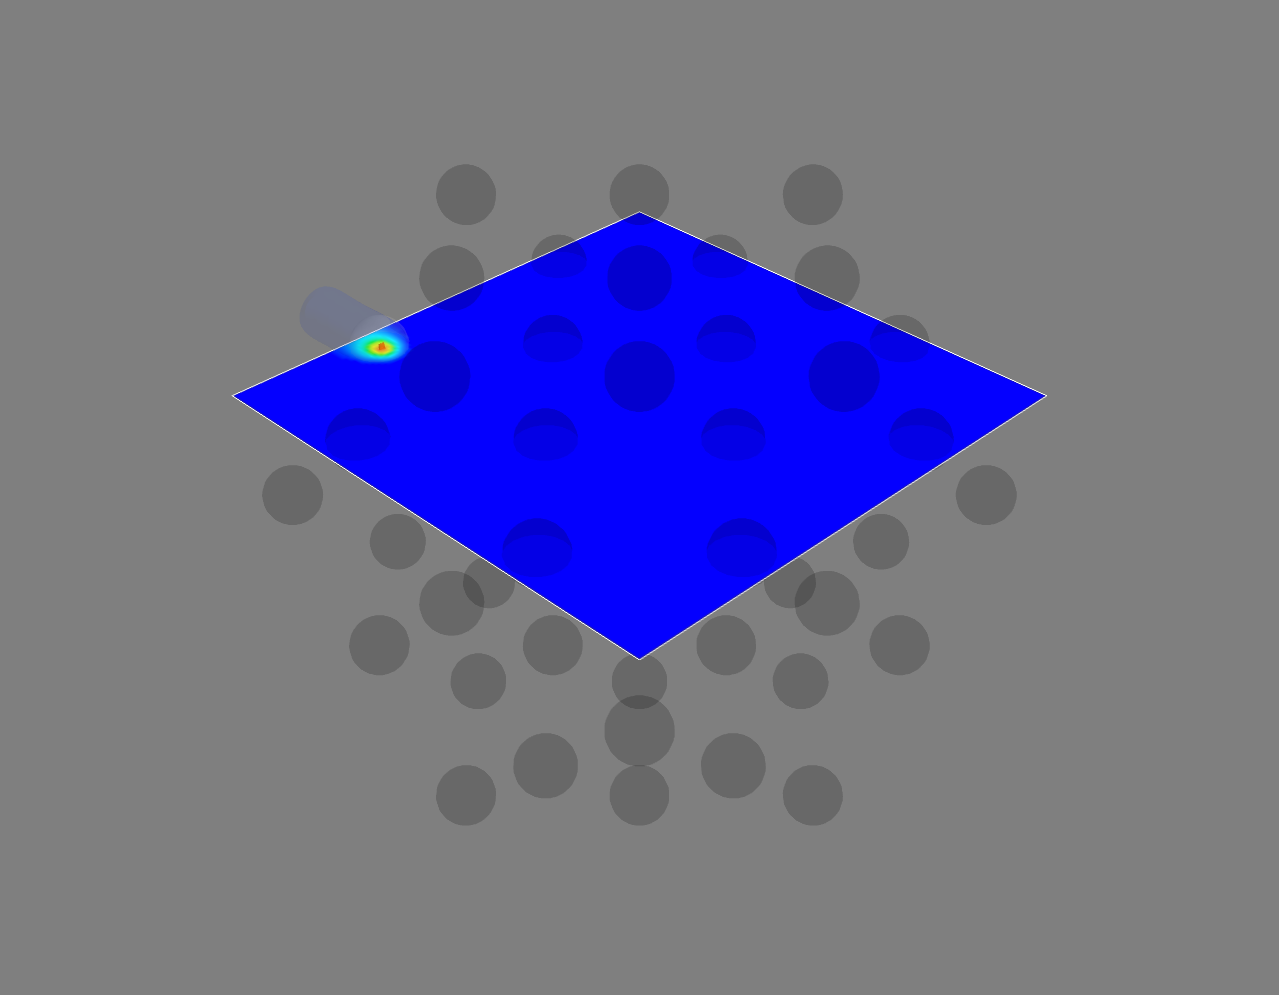
\includegraphics[width=.8\textwidth]{snapshot}\label{subfig: biasing_map}} \\
    \subfloat[]{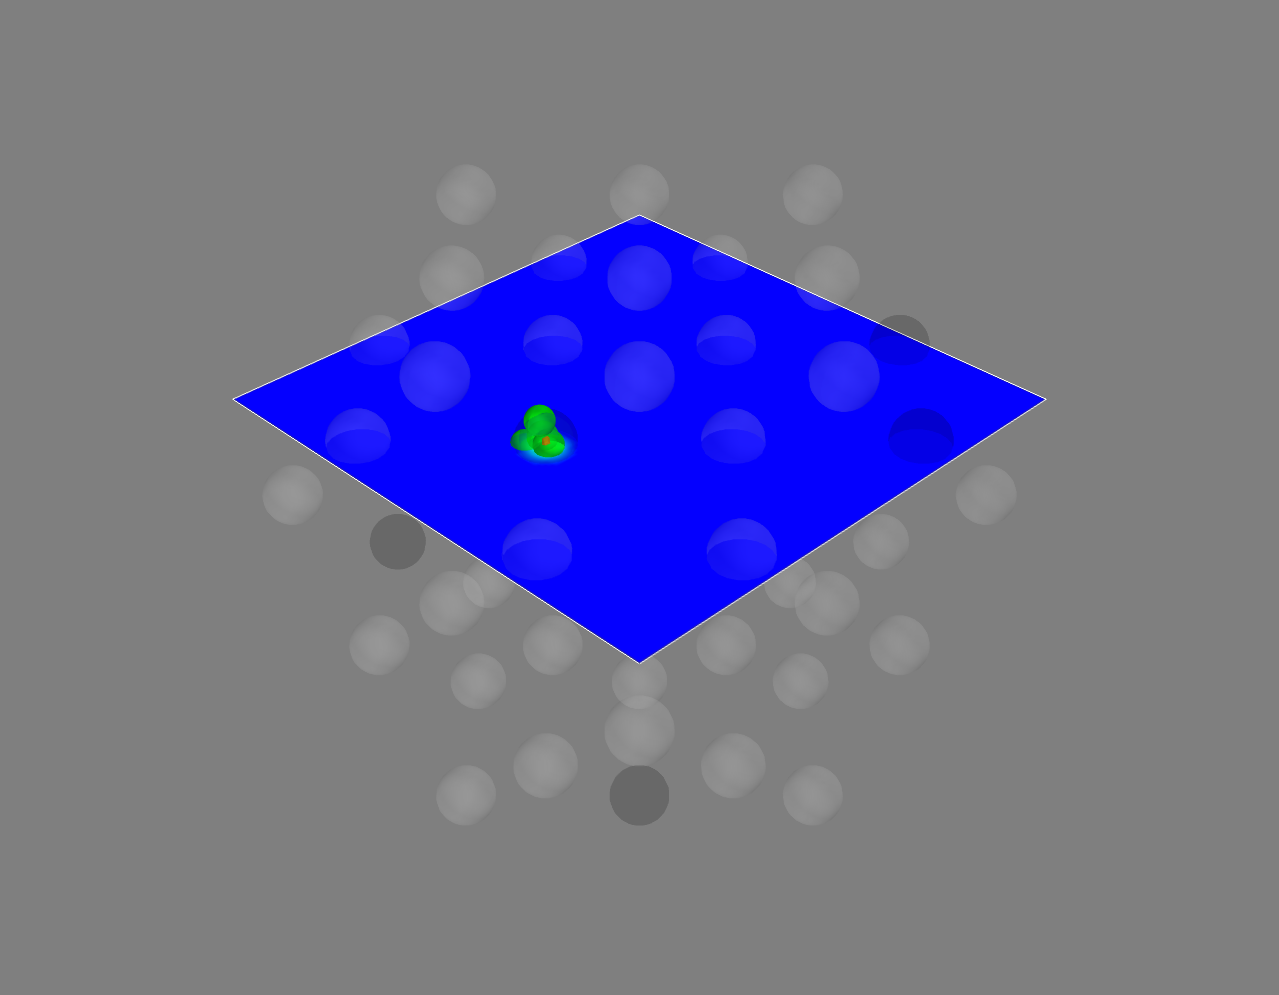
\includegraphics[width=.8\textwidth]{gc_positioning_snapshot}\label{subfig: insertian_trials}}
	\caption[Addition biasing with a Lennard Jones potential.]{These figures show slices of the three dimensional addition potential energy surface. a) shows the addition probability, with the red area most probable. b) shows the results of trial insertions, where the green spheres denote where insertions were attempted.}
	\label{fig:biasing}
\end{figure}
Figure \ref{subfig: biasing_map} shows an example map for atomic addition in a Au54 atom system, with an Au55 atom target.
Figure \ref{subfig: insertian_trials} shows the results of a few GCMC insertions with biasing, showing the focusing of the simulation on the missing atom.
The high density of insertions around the missing atom would not have been possible without the biasing.


\section{Conclusions}
In this chapter we have presented the development of both PES and the statistical mechanical ensembles used to search them.
We expanded the classical concept of a PES to a more generall mapping from positional variable space to energy space.
This expantion allowed for the implementation of experimentally derived PES, where the disagreement between experimental and computed results can be included in the PES.
Common experimental PESs were discussed, and their forces derived.
The implementation of various statistical mechanical ensembles, used for searching the PES for minima, was also discussed with a special focus on No-U-Turn-Sampling Hamiltonian Monte Carlo.
Grand Canonical Monte Carlo was also discussed, with an emphasis on the us of biasing to increase the overall acceptance rate.
Future work in this area may include the development of PESs which leverage 2 dimensional data, like STEM images, or ensembles which help to eliminate tuned parameters like parallel tempering.


\graphicspath{{./pdf/figures/}}
\graphicspath{{./pdf/figures/}}
\tikzstyle{startstop} = [rectangle, rounded corners, minimum width=3cm, minimum height=1cm,text centered, draw=black, fill=red!30]
\tikzstyle{io} = [trapezium, trapezium left angle=70, trapezium right angle=110, minimum width=3cm, minimum height=1cm, text centered, draw=black, fill=blue!30]
\tikzstyle{process} = [rectangle, minimum width=3cm, minimum height=1cm, text centered, draw=black, fill=orange!30]
\tikzstyle{decision} = [diamond, minimum width=3cm, minimum height=1cm, text centered, draw=black, fill=green!30]
\usetikzlibrary{shapes.geometric}
\tikzstyle{database} = [cylinder, minimum width=3cm, minimum height=1cm, text centered, draw=black, fill=yellow!30, shape border rotate=90, aspect=0.25]

\chapter{Atomic Pair Distribution Function: \\Theory and Computation} \label{ch:pdf}
\section{Theory}
To properly understand the PDF and its limitations we need to derive its mathematics.
The PDF has been previously derived many times so it is not re-derived here.
This discussion of the PDF and its gradients use the notation of Farrow and Billinge. \cite{Farrow2009}
\subsection{Derivation}
\section{Theory}
To properly understand the PDF and its limitations we need to derive its mathematics.
The PDF has been previously derived many times so it is not re-derived here.
This discussion of the PDF and its gradients use the notation of Farrow and Billinge. \cite{Farrow2009}
\subsection{Derivation}
Many of the above techniques require the gradient of the PES.
This in turn requires the gradient of the PDF to be derived.
Mathematically treating thermal vibrations will also be discussed in this section.
Systems which are truly extended materials, like powders with particle sizes larger than 10nm, are best formulated as systems with periodic boundaries.
Thus, the equations for a periodically bound PDF need to be developed as well, with their gradients.
\subsection{Analytically Gradients}
Many optimization algorithms and simulations methodologies, including HMC, require not only the potential energy of a given configuration but also the forces acting on that configuration.
These forces are described by the gradient of potential energy of the system which in turn requires the gradient of the PDF.
As previously shown the PDF is the Fourier Transform of the Debye equation.
Since the Fourier Transform is expressed as an integral we can exchange the order of the gradient and the integral, allowing us to calculate the analytical gradient of the Debye equation and FFT the resulting function.
The Debye equation, with a Debye-Waller vibrational correction is
\begin{equation}
F(Q) = \frac{1}{N \langle f \rangle^{2}} \sum_{j\neq i} f_i^{*}(Q)f_j(Q) \exp(-\frac{1}{2}\sigma_{ij}^{2}Q^{2}) \frac{\sin(Qr_{ij})}{r_{ij}}
\end{equation}
where
\begin{eqnarray}
  \sigma_{ij}^{2} = (\vec{u}_{ij} * \hat{d}_{ij})^{2}\\
  \vec{u}_{ij} = \vec{u}_{i} - \vec{u}_{j}\\
  \hat{d}_{ij} = \frac{\vec{d}_{ij}}{r_{ij}}\\
  r_{ij} = ||\vec{d}_{ij}|| \\
  \vec{d}_{ij} =
  \begin{bmatrix}
    q_{ix} - q_{jx}\\
    q_{iy} - q_{jy} \\
    q_{iz} - q_{jz}
  \end{bmatrix}
\end{eqnarray}
where $Q$ is the scatter vector, $f_i$ is atomic scattering factor of the $i$th atom, and $r_{ij}$ is the distance between atoms $i$ and $j$ and has $q$ dependence. \cite{Jeong2002}
For simplicity's sake we will break up $F(Q)$ so that
\begin{equation}
F(Q) = \alpha \sum_{j\neq i} \beta_{ij} \uptau_{ij} \Omega_{ij} \label{eq:abto}
\end{equation}
where
\begin{eqnarray}
  \alpha = \frac{1}{N \langle f \rangle^{2}} \label{eq:alpha} \\
  \beta_{ij} = f_i^{*}(Q)f_j(Q)\label{eq:beta}\\
  \uptau_{ij} = \exp(-\frac{1}{2}\sigma_{ij}^{2}Q^{2}) \label{eq:tau}\\
  \Omega_{ij} = \frac{\sin(Qr_{ij})}{r_{ij}} \label{eq:omega}
\end{eqnarray}

\noindent The derivatives are as follows:
\begin{equation}
\frac{\partial}{\partial q_{i,w}} F{ (Q )} = \alpha \sum_{j} \beta_{ij} (\frac{\partial \uptau_{ij}}{\partial q_{i,w}}  \Omega_{ij} + \uptau_{ij} \frac{\partial \Omega_{ij}}{\partial q_{i,w}}) \label{eq:grad_fq}
\end{equation}
where
\begin{eqnarray}
  \frac{\partial \Omega_{ij}}{\partial q_{i,w}}  = \frac{Q\cos(Qr_{ij}) - \Omega_{ij}}{r_{ij}^{2}} (q_{i,w}-q_{j,w})\\
  \frac{\partial \uptau_{ij}}{\partial q_{i,w}} = \frac{\sigma_{ij}Q^{2} \uptau_{ij}}{r_{ij}^{3}}   ((q_{i,w} - q_{j,w}) \sigma_{ij}- ( u_{i,w} - u_{j,w})r_{ij}^{2})
\end{eqnarray}

Since $\vec{u}_{ij}$ is a variable as well, we need the derivative with respect to it as well.
Thus
\begin{eqnarray}
\frac{\partial}{\partial u_{i,w}} F{ (Q )} = \alpha \sum_{j} \beta_{ij} \frac{\partial \uptau_{ij}}{\partial u_{i,w}}  \Omega_{ij}\\
\frac{\partial \uptau_{ij}}{\partial u_{i,w}} = - \frac{\sigma_{ij}Q^{2} \uptau_{ij}}{r_{ij}}  (q_{i,w} - q_{j,w})
\end{eqnarray}
\subsubsection{Without ADPs}
Without ADPs the equations simplify down to
\begin{equation}
F(Q) = \frac{1}{N \langle f \rangle^{2}} \sum_{j\neq} f_i^{*}(Q)f_j(Q) \frac{\sin(Qr_{ij})}{r_{ij}}
\end{equation}
and
 \begin{equation}
\frac{\partial}{\partial q_{i,w}} F{ (Q )} = \alpha \sum_{j} \beta_{ij} \frac{\partial \Omega_{ij}}{\partial q_{i,w}}
\end{equation}
use of these equations, when ADPs are not appropriate (like at cryogenic temperatures), greatly speeds up the computation.

\subsubsection{Periodic Boundary Conditions}
Periodic boundary conditions can be helpful when simulating extended solids or large nanoparticles. In this case all the non-crystallinity is contained within the simulation box and the box is repeated to create the longer distance peaks observed in the PDF. To perform this we can break up the Debye equation into two main parts, the part that describes the interatomic distances within the simulation box and those between boxes. Neglecting the thermal motion portion:
\begin{equation}
  F(Q) = \frac{1}{N \langle f \rangle^{2}}(\sum_{j\neq i} f_i^{*}(Q)f_j(Q) \frac{\sin(Qr_{ij})}{r_{ij}} + \sum_{i,j} f_i^{*}(Q)f_j(Q) \frac{\sin(QR_{ij})}{R_{ij}})
\end{equation}
where
\begin{eqnarray}
  R = |\vec{r} + \vec{\nu}|\\
  \vec{\nu} = \gamma_1*\vec{a} + \gamma_2*\vec{b} + \gamma_3*\vec{c}
\end{eqnarray}
where $\gamma_{i}$ is the number of copies of the simulation box in the $i$th direction, and $\vec{a}, \vec{b}, \vec{c}$ are the lattice or superlattice directions.

%\input{pdf/pbc_adp}



\section{Computation} \label{sec:comp}
Simply deriving the equations for the PDF is not enough.
The many body nature of the PDF equation make analytical solution of the structure from the PDF impossible.
Thus, the PDF must be computed from a structural candidates and compared against experimental results to evaluate the reliability of the model.

\subsection{HPC and GPUs}
To properly solve the structure of materials the PDF will need to be computed many times and checked against experimental results.
This requires computation of the PDF, potentially over many atoms.
Calculating these PDFs requires a fast, highly parallized, computational framework.
\subsubsection{GPUs and Parallelization}
\begin{figure}
    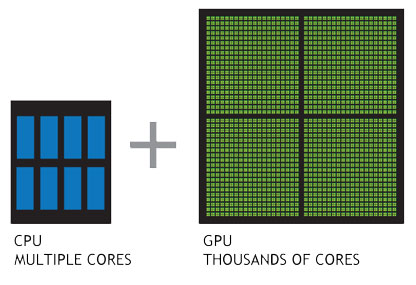
\includegraphics[width=\textwidth]{cpu-and-gpu}
    \caption{Comparison of the CPU and GPU chip architectures}
    \label{fig:cpu_vs_gpu}
\end{figure}
Computing the PDF is an embarrassingly parallel problem.
The basic procedure is to calculate the reduced structure factor $F(Q)$ for each atom pair and momentum transfer vector, sum over all the atom pairs, and Fourier transform the structure to the PDF.
The first part of this procedure is perfectly parallizable, as each atom pair is seperate from the others.
The summation over all the atomic reduced structure factors can be parallelized via distributed summing.
Lastly the FFT can be parallelized using existing parellel FFT algorithms.

GPUs are particularly well suted to the task of computing PDFs.
GPU chip architecture is designed to perform many task simultaniously by having potentially thousands of cores.

\subsubsection{Map from ij space to k space}
The above equations, although formally correct, are very ineffiecent. $F(Q)$ and its gradient are indexed over all the atoms twice, however there are symmetries that allow us to only compute over the atom pairs esentially mapping from an $n$x$n$ space, $ij$ space, to a $\frac{n(n-1)}{2}$ space, $k$ space.
For $F(Q)$ we apply the following mapping
\begin{figure}[!ht]
\begin{center}
\begin{tikzpicture}
    \node (E) at (0,0) {$E$};
    \node[right=of E] (F) {$E'$};
    \node[right=of F] (Z) {$Z$};
    \node[below=of F] (N) {$B'$};
    \node[below=of E] (M) {$B$};
    \draw[->] (E)--(F) node [midway,above] {$\psi$};
    \draw[->] (F)--(Z) node [midway,above] {$\Sigma$};
    \draw[->] (M)--(N) node [midway,below] {$\psi'$};
    \draw[->] (E)--(M) node [midway,left] {$\phi$};
    \draw[->] (N)--(Z) node [midway,left] {$\Sigma'$};
\end{tikzpicture}
\end{center}
\end{figure}
where $E$ denotes the atomic coordinates in $ij$ space, $E'$ denotes $F(Q)$ before the summation in $ij$ space, $B$ denotes the atomic pairs in $k$ space, $B'$ denotes $F(Q)$ in $k$ space, and $Z$ denotes the final summed $F(Q)$.  For the operators, $\phi$ denotes the mapping from $ij$ space to $k$ space $k = j + i * \frac{i - 1}{2}$, $\psi$ and $\psi'$ denote the $F(Q)$ operation in $ij$ and $k$ space, respectivly. $\Sigma$ denotes the sum over all the atoms.  

To properly define $\Sigma'$ we must establish whether $F(Q)$ is an even function.  
We can accomplish this by examining each of the portions of $F(Q)$, $\alpha, \beta ,\uptau, \Omega$.
$\Omega$ is even, since $r_{ij}$ is the interatomic distance, which is the same despite a flip of indicies, $Q$ does not depend on the atomic indicies, and since $Qr_{ij}$ is even so is $\sin{Qr_{ij}}$.  Thus, $\Omega$ is even.  Providing similar analysis to $\uptau$ we can see that while $\vec{u}_{ij}$ is odd, so is the unit displacement vector between the two atoms, thus the two odds cancel out.
Intuitivly this makes sense, since the $F(Q)$ equation is fundamentally interested in the interatomic distances which is even.  Thus, switching atom indicies does not change $F(Q)$.
Due to the even nature of the $F(Q)$ operator the $\Sigma'$ operator sums over all the atom pairs, and multiplies by two to reflect the double counting of the $\Sigma$ operator.

For the gradient a similar mapping is used:
\begin{figure}[h!]
\begin{center}
  \begin{tikzpicture}
    \node (E) at (0,0) {$E$};
    \node[right=of E] (F) {$E'$};
    \node[right=of F] (Z) {$Z$};
    \node[below=of F] (N) {$B'$};
    \node[below=of E] (M) {$B$};
    \draw[->] (E)--(F) node [midway,above] {$\psi$};
    \draw[->] (F)--(Z) node [midway,above] {$\Sigma$};
    \draw[->] (M)--(N) node [midway,below] {$\psi'$};
    \draw[->] (E)--(M) node [midway,left] {$\phi$};
    \draw[->] (N)--(Z) node [midway,left] {$\tilde{\phi}\Sigma$};
\end{tikzpicture}
\end{center}
\end{figure}

In this mapping, however, we use the $\tilde{\phi}\Sigma$ operator.  This operator simultaniously performs a reverse mapping from $k$ to $ij$ space, and a summation with the correct symmetry.  In this case the $\psi$ and $\psi'$ operators, which denote the $\grad{F(Q)}$ operator in $ij$ and $k$ space, are antisymmetric.  Intuitivly this makes sense as an extension of Newton's Second Law, since each particle's interation is felt oppositely by its partner.
\subsubsection{GPU Memory Allocation}
While GPUs are very fast computational engines they tend to be memory bound.
While a gradient array for a 10nm Au nanoparticle, consisting of 31,000 atoms and half a billion unique distances, occupies 1.5 TB of memory a single GPU's RAM allotment varies from 4GB on a NVIDIA GTX970 to 24 GB on a NVIDIA Tesla K80.
Thus, it is important to determine exactly how many atoms can fit on a GPU of arbitrary size as a funciton of the number of atoms and the $Q$ range.
The memory required per array is:
\begin{eqnarray}
    q [=] 3n\\
    d [=] 3k\\
    r [=] k\\
    scatter [=] nQ\\
    normalization [=] kQ\\
    omega [=] kQ\\
    F_{k}(Q) [=] kQ\\
    Sum [=] kQ\\
    Sum2 [=] kQ\\
    F(Q) [=] Q
\end{eqnarray}
where $n$ is the number of atoms, $k$ is the number of uniqe distances, $Q$ is the scatter vector.
Each of the above arrays are used in the computation and thus must be able to be held in memory.
Thus the number of atom pairs that can fit on a GPU with $am$ bytes of available memory is:
\begin{equation}
    k_{per GPU} = \frac{1}{16 Q + 16} \left(- 4 Q n - 4 Q + am - 12 n\right)
\end{equation}
If ADPs ar eincluded in the calculation, then the following arrays are also added to the memory allocaiton:
\begin{eqnarray}
    adps = 3n\\
    sigma = k\\
    tau = kQ
\end{eqnarray}
Thus the pair allotment is:
\begin{equation}
    k_{per GPU} = \frac{- 4 Q n - 4 Q + am - 24 n}{20 Q + 20}
\end{equation}

For the Gradient we need to calculate $F(Q)$ and its gradient, so the total memeory overhead is equal to the previously mentioned arrays plus:
\begin{eqnarray}
    g_omega = 3kQ \\
    g_fq = 3kQ \\
    rtn = 3nQ
\end{eqnarray}
Thus the gradient allotment is:
\begin{equation}
    \grad{k_{per GPU}} = \frac{- 16 Q n + am - 12 n}{32 Q + 16}
\end{equation}
For the gradient with ADPs the ADP gradient array is:
\begin{equation}
    g_tau = 3kQ
\end{equation}
Thus the allocation is:
\begin{equation}
    \grad{k_{per GPU}} = \frac{ - 16 Q n + am - 24 n}{48 Q + 20}
\end{equation}
These equations were solved by sympy as their validity is very important to the overal relyability of the software.
If the GPU is overallocated then the system may crash or return meaningless results.

\todo[inline]{Include Speed Benchmarks Here}

\graphicspath{{./bmk/figures/}}
\chapter{Benchmarking} \label{ch:bmk}
\todo[inline]{This entire section needs some rewritting to distinguish this from the paper}
\todo[inline]{Also some introduction would be great}
\todo[inline]{this just needs a lot of work}
\section{Introduction}
The NUTS-HMC system was tested on a series of nanoparticle (NP) benchmarks.
The purpose of these benchmarks is to test the ability of the NUTS-HMC system to reproduce the target PDF and its associated structure.
Systems were chosen for their size, crystallinity, and interfacial differences.

\section{PDF}
The formation of NPs with both crystallographic and non-crystallographic structures \cite{Marks1994} and with different chemical patterns \cite{Ferrando2008} are well documented.
For simplicity, we chose monometallic Au clusters as benchmarks and considered two groups of structures with different size and degrees of structural disorder in order to assess the reliability and efficiency of our HMC method for solving atomic structures from PDFs.
The first group consists of \ce{Au55} clusters with different degrees of disorder, including a crystalline cluster structure in $O_h$ (Octahedral) symmetry, a structure with a disordered surface, and an amorphous structure.
The second group consists of the crystallographically solved \ce{Au102} structure as in the \ce{Au102MBA44} nanocrystals \cite{Jadzinsky2007,Li2008}.
We used optimized structures from the Density Functional Theory (DFT) as target structures and generated the corresponding PDF, $G_{_\mathrm{obs}}$, according to
\begin{equation}
\label{Eq:Gdef}
  G_{_\mathrm{obs}} = \frac{2}{\pi} \int_{Q_\mathrm{min}}^{Q_\mathrm{max}} Q[S_{_\mathrm{obs}}(Q) - 1] \sin{\left (Q r \right )}\, dQ
\end{equation}
where $S_{_\mathrm{obs}}$ is the target structure's structure factor.
Since all the target structures were optimized by DFT at zero Kelvin the target and model PDF profiles were calculated at zero temperature, with no atomic displacement parameters (ADPs).
However, ADPs would have a considerable impact on the calculation of the PDF, especially for nanoparticles at non-zero temperatures.


Spin-polarized  DFT calculations were carried out using the Vienna ab initio simulation package (VASP) \cite{Kresse1993, Kresse1994} within the  Perdew-Burke-Ernzerhof (PBE) exchange-correlation functional \cite{PERD1996}.
The projected augmented wave method \cite{Blochl1994} and a kinetic energy cutoff of 400 eV were used.
Structural optimization was performed until the total energy and ionic forces were converged to 10$^{-6}$ eV and 10 meV/\AA, respectively.
The  amorphous \ce{Au55} structures were generated by simulated annealing using the classical embedded atom method potential \cite{Sheng2011}.
Different annealing temperatures between 1200 K and 1670 K (bulk melting temperature of Au) were used and the thermally equilibrated structures were cooled down to 300 K before minimization at 0 K.
Further optimization using DFT leads to total energies that vary within 1-2 eV among different amorphous structures  and the lowest energy one was used as the target structure. The target structure of \ce{Au102} was taken as the \ce{Au102} core of the DFT-optimized \ce{Au102MBA44} cluster \cite{Li2008}.

All systems were refined using a PES  which consists of a linear combination of $Rw$, the repulsive and attractive thresholded spring potentials.  The total potential energy in the Hamiltonian in Eq. (\ref{Hamiltonian}) is expressed as:
\begin{eqnarray}\label{eq:Ucomp}
  U(q) = U_{Rw}(q) + U_\mathrm{spring}(q, R_\mathrm{min}) + U_\mathrm{spring}(q, R_\mathrm{max})
\end{eqnarray}
The thresholded spring potentials are based on those previously proposed on by Peterson \cite{Peterson2014}, i.e.  $U_\mathrm{spring}(q, r_{t}) = \frac{\kappa}{2}\sum_{i, j}(r_{i, j}-r_t)^{2}$  for all atomic distance $r_{i,j}$  outside the bounds of the spring threshold $r_t$.
The resulting restoring forces on the out-of-bound atoms  bring the system back within the bounds of the PDF, $R_\mathrm{min}$ and $R_\mathrm{max}$, and therefore preventing the system from exploding or collapsing.
Otherwise,  incorrect refinements may result by having atomic pair distances out of the PDF bounds.  $\kappa$ is the spring constant in eV/\AA~and the $Rw$ potential is converted from unitless to eV via multiplication by a conversion factor $\lambda$.

Whereas the choice of the absolute values of $\lambda$ and $\kappa$ is somewhat arbitrary, their relative values are important in determining which  term in Eq.~(\ref{eq:Ucomp}) dominates the PES, especially when considering the effect of the simulation temperature.
Generally, the ratio between the total potential energy and the temperature determines how much random motion will dominate the dynamics; a lower ratio implies that random motion will play a large role in the dynamics.
The ratio between $\lambda$ and $\kappa$ of each spring describes how far the PDF can push the system below or above the bounds set by the spring potentials.
Heuristically, too stiff a spring  forbids the system to access new configurations, e.g.  high energy ``transition states'' which may involve shorter bonds or a larger system size.
Conversely, too small a spring constant makes it slower for the system to snap back within bounds and may lead to an explosion or implosion of the system, leaving the dynamics to drift aimlessly.

\subsection{Model Parameters}
Unless otherwise stated, the PDFs of the target and starting structures were generated using Eqn. (\ref{Eq:Gdef}) with a step of $\delta R=.01$~\AA, $Q_\mathrm{min}=0.1$~\AA$^{-1}$,  $Q_\mathrm{max}=25.0$~\AA$^{-1}$.
$R_\mathrm{min}$ and $R_\mathrm{max}$ correspond to the first minimum before the first PDF peak and that after the last PDF peak, respectively, which ensure that the full meaningful region of the PDF is modeled.  For each of the simulations, the Q resolution was calculated by
\begin{equation}
\delta Q=\frac{\pi} {R_\mathrm{max} + \frac{12 \pi}{Q_\mathrm{max}}}
\end{equation}

The HMC simulation was run with $N=300$  iterations, a target acceptance rate of 0.65, and an average starting momentum for each NUTS iteration  of 10 eVfs/\AA. Both  repulsive and attractive spring potentials are used with $\kappa=200$ eV/\AA ~and thresholds matching $R_\mathrm{max}$ and $R_\mathrm{min}$ of the PDF, respectively.  $\lambda=$ 300 eV was used as conversion factor for $Rw$. Each simulation was run with a pair of Nvidia GTX970 graphics cards, with one card partially occupied with desktop visualization.


\foreach \n in {au55sr, au55sd, au55a, au102tp, au147}{
    \input{bmk/\n}
}

\section{PDF with ADPs}
\foreach \n in {adp_50
%, adp_random, adp_janus
}{
    \input{bmk/\n}
}
\begin{enumerate}
\item Basic 50\% larger magnitude
\item Random addition to APDs
\item Janus ADPs
\end{enumerate}

\chapter{Annealing and Aggregation of 2nm \\\ce{Au} Nanoparticles}
\section{Experiments}
\subsection{NP Synthesis}
\subsection{X-ray Total Scattering Measurements}
\section{Data Processing}
\section{Data Analysis}
\section{Simulation}
\section{Structural Analysis}
\section{Conclusions}

\chapter{Phase Changes and Annealing Dynamics of \ce{Pr2NiO4} and its derivatives}
\section{Experiments}
\subsection{\ce{Pr2NiO4} Synthesis}
\subsection{X-ray Total Scattering Measurements}
\section{Data Processing}
\section{Data Analysis}
\subsection{Intra Sample Comparison}
\subsection{Inter Sample Comparison}
\section{Simulation}
\subsection{Small Box}
\subsection{Large Box}
\section{Structural Analysis}
\section{Conclusions}

\chapter{Conclusion}
%\include{Conclusion}     %% Honors theses are required to 
                          %% have an unnumbered chapter
                          %% for conclusions.  The file
                          %% Conclusion.tex should begin
                          %%   
                          %% \chapter*{Conclusion}
                          %% followed by the appropriate
                          %% text.

% \printbibliography %%  This is the command to use to
			       %%  insert the bibliography if you are using
                           %% the biblatex.sty package.  See the 
                           %% uscthesisdoc.pdf documentation for
                           %% for alternative bibliographic systems.     

\Appendix                 %% Use this command if you have one 
                          %% appendix. Use \Appendices if you 
                          %% have more than one.
	
% \input{toolong}         %% Calls toolong.tex which contains
                          %% an appendix. After issuing the 
                        %% command \Appendix or \Appendices
                        %% you must use \input not \include
                        %% to load the first appendix.

\end{document}
%%%%%%%%%%%%%%%%%%%%%%%%%%%%%%%%%%%%%%%%%%%%%%%%%%%%%%%%%%%%%%%
